%% LyX 2.1.3 created this file.  For more info, see http://www.lyx.org/.
%% Do not edit unless you really know what you are doing.

\documentclass[english]{beamer}
\usepackage[T1]{fontenc}
\usepackage[latin9]{inputenc}
\usepackage{amsmath}
\usepackage{listings}


\makeatletter
%%%%%%%%%%%%%%%%%%%%%%%%%%%%%% Textclass specific LaTeX commands.
 % this default might be overridden by plain title style
 \newcommand\makebeamertitle{\frame{\maketitle}}%
 % (ERT) argument for the TOC
 \AtBeginDocument{%
   \let\origtableofcontents=\tableofcontents
   \def\tableofcontents{\@ifnextchar[{\origtableofcontents}{\gobbletableofcontents}}
   \def\gobbletableofcontents#1{\origtableofcontents}
 }

%%%%%%%%%%%%%%%%%%%%%%%%%%%%%% User specified LaTeX commands.
\usetheme{Rochester}
\usecolortheme{beaver}

\usenavigationsymbolstemplate{}
\setbeamercolor{structure}{fg=darkred}
\setbeamercolor{block body}{bg=gray!10!white}

\makeatother

\usepackage{babel}
\begin{document}
\title{Accelerating your Python Code}
\subtitle{For GMMs with PyCUDA}

\author{Varun Nayyar}


\date{27/07/18}
\makebeamertitle

\begin{frame}[t]\frametitle{Outline}
Me = Math Major + Script Kiddy (Manage Expectations)
 
\begin{block}{What to Expect}
  \begin{itemize}
    \item Some Math
    \item Thinking with CUDA and Basic Syntax
    \item How to use PyCUDA to avoid complicated work
  \end{itemize}

\end{block}

\begin{block}{What NOT to Expect}
  \begin{itemize}
    \item How PyCUDA does it's magic
    \item Intermediate/Advanced CUDA
  \end{itemize}
\end{block}


\end{frame}



\begin{frame}[t]\frametitle{Gaussian Mixture Models d=1, K=2}
    \begin{center}
        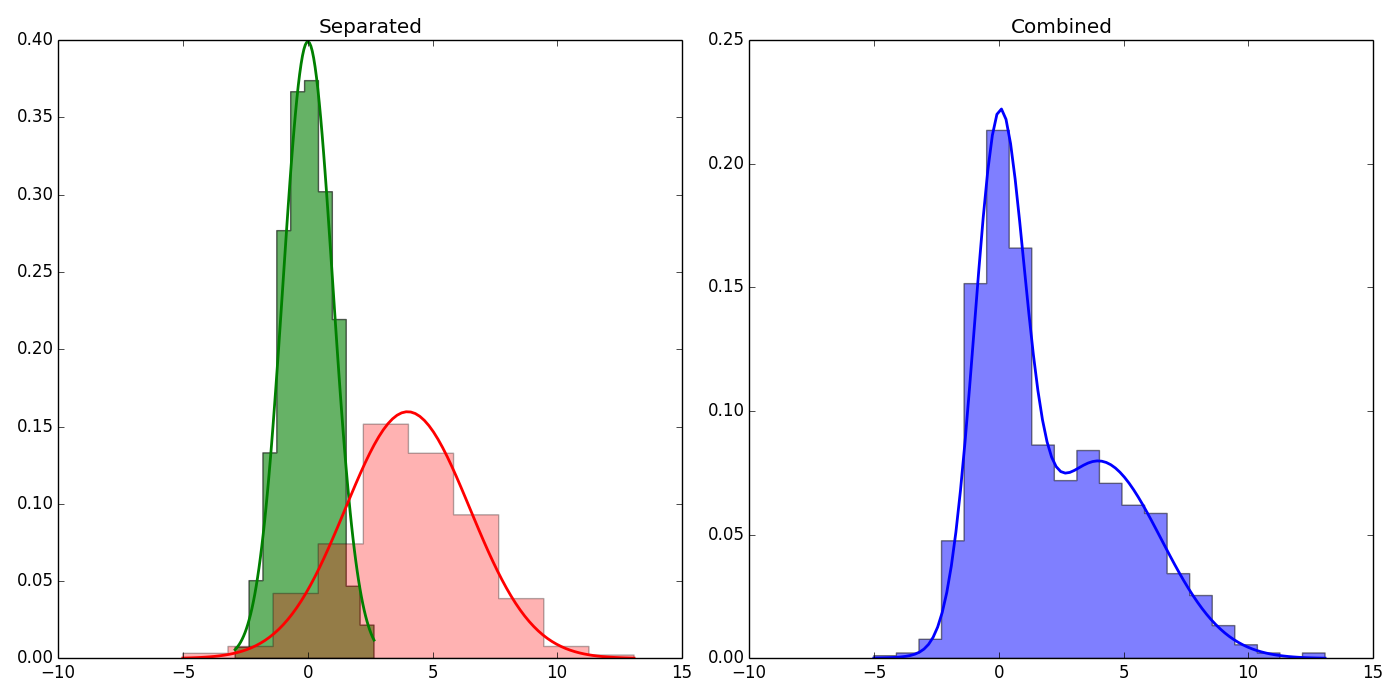
\includegraphics[width=10cm]{img/Combined.png}
    \end{center}
K-means+=1
\end{frame}


\begin{frame}[t]\frametitle{Gaussian Mixture Models (GMMs)}
\begin{block}{Density Function}
For $K$ mixtures
\begin{align*}
f(\mathbf{x}|\boldsymbol{\pi},\boldsymbol{\mu},\boldsymbol{\Sigma})= & \sum_{k=1}^{K}\pi_{k}\mathcal{N}(\mathbf{x}|\mu_{k},\Sigma_{k}) 
\end{align*}
\end{block}

\begin{block}{Log Likelihood (function of concern)}
  \begin{align*}
  l(\mu,\Sigma,\mathbf{x})  = &\sum_{i=1}^{N}\ln\left(\sum_{k=1}^{K}\pi_{k}\mathcal{N}(x_{i}|\mu_{k},\Sigma_{k})\right)\label{eq:LogLikelihood}
  \end{align*}
\end{block}

\end{frame}


\begin{frame}[t]\frametitle{Need for speed}
Some post-hoc realizations
\begin{itemize}
    \item GMM likelihood formula doesn't decompose into a mathematically simple form
    \item However, note that the GMM likelihood has a parallelizable form in that each point of each mixture is independent (CUDA vibes)
\end{itemize}
Computational Numbers
\begin{itemize}
    \item Number of flops are of the order of $O(NKd)$, in my case, $N = 10^6$, $K = 8$, $d = 13$. I.e. $O(10^8)$
    \item I needed to evaluate the likelihood $10^6$ times for a fixed dataset while the parameters were varied. (Markov Chain Monte Carlo)
    \item i.e $10^{14}$ floating point operations per run.
\end{itemize}        
\end{frame}

\begin{frame}[t]\frametitle{First Attempt}

\begin{columns}

  \column{0.5\textwidth}
    \begin{itemize}
      \item Eh, my computer is fast enough
      \item Pure Python (numpy)
      \item Averaged 36 us per datapoint, or 36s for whole dataset
      \item $10^6$ evaluations would take ~1 year
    \end{itemize}


  \column{0.5\textwidth}
    \begin{center}
        
\includegraphics[height=6cm]{img/doingitlive.jpg}
    \end{center}

\end{columns}

\end{frame}


\begin{frame}[t]\frametitle{Execution speed per N}
    \begin{center}
        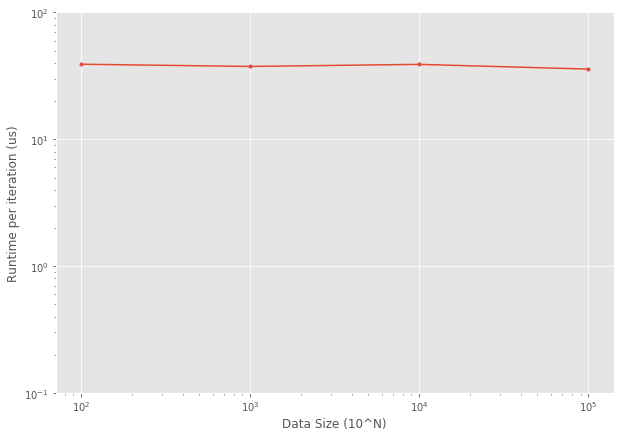
\includegraphics[width=10cm]{img/simpleOnly.png}
    \end{center}
\end{frame}


\begin{frame}[t]\frametitle{Second Attempt}

\begin{columns}

  \column{0.5\textwidth}

    \begin{itemize}
      \item Stand on the shoulders of giants (scikit-learn)
      \item Reverse engineered the likelihood evaluator
      \item 72x improvement!
      \item Took 0.5 us per datapoint, or 0.5s for whole dataset
      \item $10^6$ evaluations would take ~5 days!
    \end{itemize}


  \column{0.5\textwidth}
    \begin{center}
        
\includegraphics[width=4cm,height=6cm]{img/shoulders.jpg}
    \end{center}
\end{columns}

\end{frame}


\begin{frame}[t]\frametitle{Execution speed per N}
    \begin{center}
        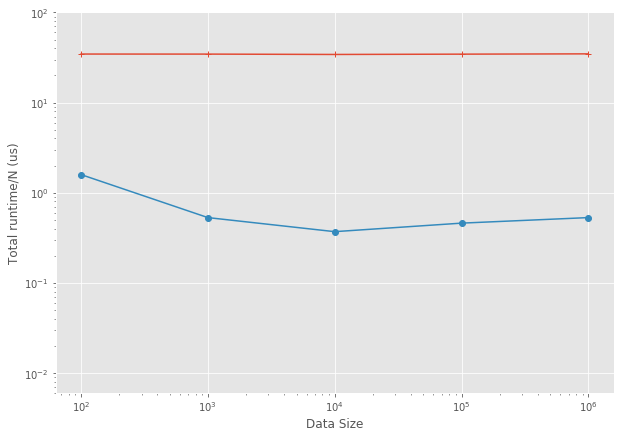
\includegraphics[width=10cm]{img/skandsimple.png}
    \end{center}
\end{frame}


\begin{frame}[t]\frametitle{Aside: Timing Methodology and Testing}
\begin{itemize}
    \item fixed $K=8$ and $d=13$ as per live behaviour. Varied $N$ from $10^2$ to $10^6$ for completeness. $10^6$ is intended data size.
    \item Used \texttt{timeit} module with 100 iterations and report totaltime/$100*N$
\end{itemize}
Testing
\begin{itemize}
    \item Manually compared my hand written version to R implementation using output
    \item Used \texttt{pytest} to create random tests to check that random data and parameters matched values.
\end{itemize}
It's good to be rigorous - Math Major
\end{frame}


\begin{frame}[t]\frametitle{CUDA}
  \begin{itemize}
    \item Stood for Compute Unified Device Architecture but no one cared so this was forgotten
    \item CUDA devices have Streaming Multiprocessors (SMs) and each has a number of CUDA cores. CUDA runs threads in batches of 32 called Warps. GTX970 has 13 SMs with 128 CUDA cores each.
    \item in the CUDA paradigm, you need plenty of independent threads to take advantage of the architecture and to minimize memory latency via async scheduling.
    \item Not many guarantees of all threads running exactly in parallel, so code still needs to be thread safe. 
    \item number of threads is magnitudes greater than in standard multicore programming. 
  \end{itemize}

\end{frame}

\begin{frame}[t]\frametitle{Thinking with CUDA (Matrix Multiplication)}

\begin{align*}
\left(\begin{array}{cccc}
a_{11} & a_{12} & \cdots & a_{1n}\\
\\
\vdots &  & \ddots\\
a_{n1} &  &  & a_{nn}
\end{array}\right) &\times \left(\begin{array}{cccc}
b_{11} & b_{12} & \cdots & b_{1n}\\
\\
\vdots &  & \ddots\\
b_{n1} &  &  & b
\end{array}\right)
\end{align*}
  \begin{itemize}
    \item <1->Each element on output matrix requires $n$ multiplications and additions. $n^2$ elements. 
    \item <1->Single Core = $O(n^3)$, though tricks allow for $O(n^{2.81})$
    \item<1> CUDA??
    \item<2-> Theoretical CUDA = $O(n)$
    \item<3-> Create $n^2$ threads. Each takes $O(n)$ time and can be run in parallel

  \end{itemize}

\end{frame}

\begin{frame}[t]\frametitle{Thinking with CUDA (Summing an Array)}

Sum an array $\left(\begin{array}{cccc} a_{1} & a_{2} & \cdots & a_{n}\end{array}\right)$

  \begin{itemize}
    \item<1-> Single Core = $O(n)$
    \item<1> CUDA ??
    \item<2-> theoretical CUDA = $O(lg (n))$
    \item<3-> First pass, have $N/2$ threads add pos $i$ and pos $i+N/2$
    \item<3-> Second pass, have $N/4$ threads add pos $i$ and pos $i+N/4$

  \end{itemize}

\end{frame}


\begin{frame}[t]\frametitle{Thinking with CUDA (Summing an Array)}

Sum an array $\left(\begin{array}{cccc} a_{1} & a_{2} & \cdots & a_{n}\end{array}\right)$

  \begin{itemize}
    \item<1-> Single Core = $O(n)$
    \item<1> CUDA ??
    \item<2-> theoretical CUDA = $O(lg (n))$
    \item<3-> First pass, have $N/2$ threads add pos $i$ and pos $i+N/2$
    \item<3-> Second pass, have $N/4$ threads add pos $i$ and pos $i+N/4$

  \end{itemize}

\end{frame}

\begin{frame}[t]\frametitle{CUDA Architecture}

    \begin{center}
        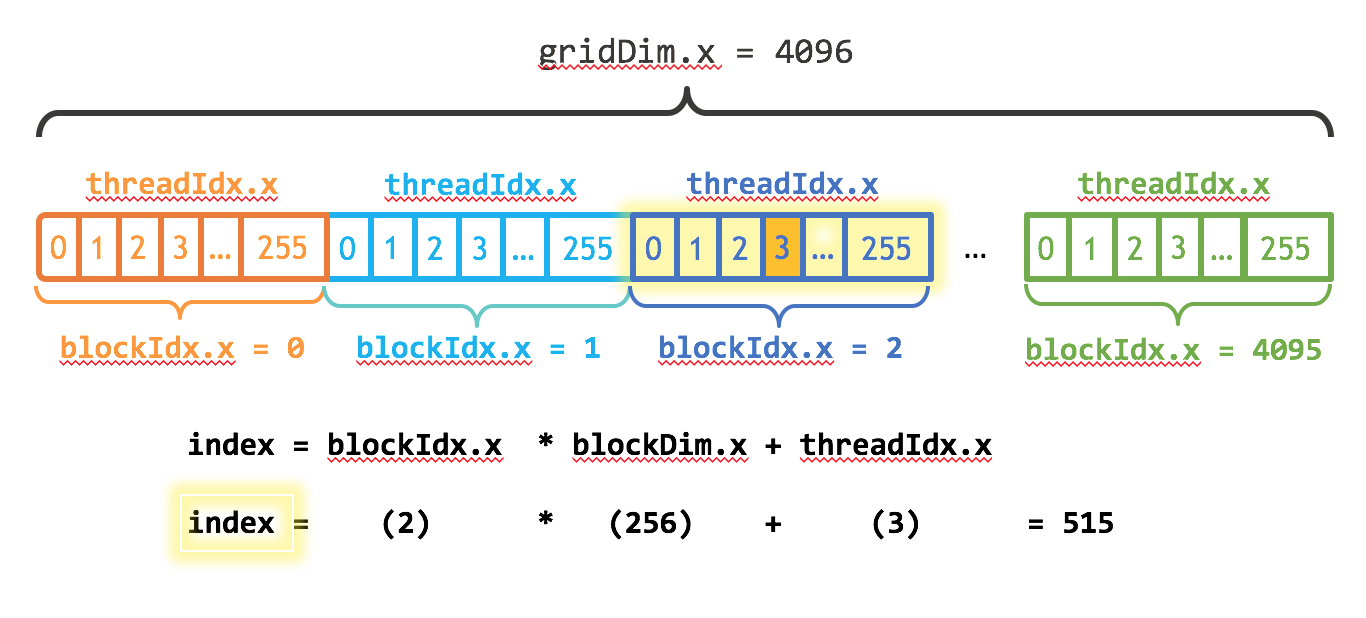
\includegraphics[width=12cm]{img/cudamodel.png}
    \end{center}

\end{frame}

\begin{frame}[t]\frametitle{CUDA Architecture}

  \begin{itemize}
    \item We have a grid of blocks and blocks of threads. 
    \item Note that the grid, blocks and threads can be 3d if necessary, but for simplicity we will only consider 1d blocks and threads and a single grid.
    \item Each block runs 32 threads at a time (called warps) and shares a limited amount of memory available to all threads (usually 48kB)
    \item GTX 970 = 128 cores * 13 SMs = 52 concurrent warps can run.
    \item Threads act asynchronously - when they access data, threads give up resources while waiting for data.
    \item memory access and data transfers (especially between host and device) have a lot of tricks and patterns to optimize (none of which I'm going to investigate)

  \end{itemize}

\end{frame}



\end{document}

